\PassOptionsToPackage{unicode=true}{hyperref} % options for packages loaded elsewhere
\PassOptionsToPackage{hyphens}{url}
%
\documentclass[]{article}
\usepackage{lmodern}
\usepackage{amssymb,amsmath}
\usepackage{ifxetex,ifluatex}
\usepackage{fixltx2e} % provides \textsubscript
\ifnum 0\ifxetex 1\fi\ifluatex 1\fi=0 % if pdftex
  \usepackage[T1]{fontenc}
  \usepackage[utf8]{inputenc}
  \usepackage{textcomp} % provides euro and other symbols
\else % if luatex or xelatex
  \usepackage{unicode-math}
  \defaultfontfeatures{Ligatures=TeX,Scale=MatchLowercase}
\fi
% use upquote if available, for straight quotes in verbatim environments
\IfFileExists{upquote.sty}{\usepackage{upquote}}{}
% use microtype if available
\IfFileExists{microtype.sty}{%
\usepackage[]{microtype}
\UseMicrotypeSet[protrusion]{basicmath} % disable protrusion for tt fonts
}{}
\IfFileExists{parskip.sty}{%
\usepackage{parskip}
}{% else
\setlength{\parindent}{0pt}
\setlength{\parskip}{6pt plus 2pt minus 1pt}
}
\usepackage{hyperref}
\hypersetup{
            pdftitle={Assignment 2 - Integer Linear Programming},
            pdfauthor={Sanja Stanisic, n. 800409},
            pdfborder={0 0 0},
            breaklinks=true}
\urlstyle{same}  % don't use monospace font for urls
\usepackage[margin=1in]{geometry}
\usepackage{color}
\usepackage{fancyvrb}
\newcommand{\VerbBar}{|}
\newcommand{\VERB}{\Verb[commandchars=\\\{\}]}
\DefineVerbatimEnvironment{Highlighting}{Verbatim}{commandchars=\\\{\}}
% Add ',fontsize=\small' for more characters per line
\usepackage{framed}
\definecolor{shadecolor}{RGB}{248,248,248}
\newenvironment{Shaded}{\begin{snugshade}}{\end{snugshade}}
\newcommand{\AlertTok}[1]{\textcolor[rgb]{0.94,0.16,0.16}{#1}}
\newcommand{\AnnotationTok}[1]{\textcolor[rgb]{0.56,0.35,0.01}{\textbf{\textit{#1}}}}
\newcommand{\AttributeTok}[1]{\textcolor[rgb]{0.77,0.63,0.00}{#1}}
\newcommand{\BaseNTok}[1]{\textcolor[rgb]{0.00,0.00,0.81}{#1}}
\newcommand{\BuiltInTok}[1]{#1}
\newcommand{\CharTok}[1]{\textcolor[rgb]{0.31,0.60,0.02}{#1}}
\newcommand{\CommentTok}[1]{\textcolor[rgb]{0.56,0.35,0.01}{\textit{#1}}}
\newcommand{\CommentVarTok}[1]{\textcolor[rgb]{0.56,0.35,0.01}{\textbf{\textit{#1}}}}
\newcommand{\ConstantTok}[1]{\textcolor[rgb]{0.00,0.00,0.00}{#1}}
\newcommand{\ControlFlowTok}[1]{\textcolor[rgb]{0.13,0.29,0.53}{\textbf{#1}}}
\newcommand{\DataTypeTok}[1]{\textcolor[rgb]{0.13,0.29,0.53}{#1}}
\newcommand{\DecValTok}[1]{\textcolor[rgb]{0.00,0.00,0.81}{#1}}
\newcommand{\DocumentationTok}[1]{\textcolor[rgb]{0.56,0.35,0.01}{\textbf{\textit{#1}}}}
\newcommand{\ErrorTok}[1]{\textcolor[rgb]{0.64,0.00,0.00}{\textbf{#1}}}
\newcommand{\ExtensionTok}[1]{#1}
\newcommand{\FloatTok}[1]{\textcolor[rgb]{0.00,0.00,0.81}{#1}}
\newcommand{\FunctionTok}[1]{\textcolor[rgb]{0.00,0.00,0.00}{#1}}
\newcommand{\ImportTok}[1]{#1}
\newcommand{\InformationTok}[1]{\textcolor[rgb]{0.56,0.35,0.01}{\textbf{\textit{#1}}}}
\newcommand{\KeywordTok}[1]{\textcolor[rgb]{0.13,0.29,0.53}{\textbf{#1}}}
\newcommand{\NormalTok}[1]{#1}
\newcommand{\OperatorTok}[1]{\textcolor[rgb]{0.81,0.36,0.00}{\textbf{#1}}}
\newcommand{\OtherTok}[1]{\textcolor[rgb]{0.56,0.35,0.01}{#1}}
\newcommand{\PreprocessorTok}[1]{\textcolor[rgb]{0.56,0.35,0.01}{\textit{#1}}}
\newcommand{\RegionMarkerTok}[1]{#1}
\newcommand{\SpecialCharTok}[1]{\textcolor[rgb]{0.00,0.00,0.00}{#1}}
\newcommand{\SpecialStringTok}[1]{\textcolor[rgb]{0.31,0.60,0.02}{#1}}
\newcommand{\StringTok}[1]{\textcolor[rgb]{0.31,0.60,0.02}{#1}}
\newcommand{\VariableTok}[1]{\textcolor[rgb]{0.00,0.00,0.00}{#1}}
\newcommand{\VerbatimStringTok}[1]{\textcolor[rgb]{0.31,0.60,0.02}{#1}}
\newcommand{\WarningTok}[1]{\textcolor[rgb]{0.56,0.35,0.01}{\textbf{\textit{#1}}}}
\usepackage{graphicx,grffile}
\makeatletter
\def\maxwidth{\ifdim\Gin@nat@width>\linewidth\linewidth\else\Gin@nat@width\fi}
\def\maxheight{\ifdim\Gin@nat@height>\textheight\textheight\else\Gin@nat@height\fi}
\makeatother
% Scale images if necessary, so that they will not overflow the page
% margins by default, and it is still possible to overwrite the defaults
% using explicit options in \includegraphics[width, height, ...]{}
\setkeys{Gin}{width=\maxwidth,height=\maxheight,keepaspectratio}
\setlength{\emergencystretch}{3em}  % prevent overfull lines
\providecommand{\tightlist}{%
  \setlength{\itemsep}{0pt}\setlength{\parskip}{0pt}}
\setcounter{secnumdepth}{0}
% Redefines (sub)paragraphs to behave more like sections
\ifx\paragraph\undefined\else
\let\oldparagraph\paragraph
\renewcommand{\paragraph}[1]{\oldparagraph{#1}\mbox{}}
\fi
\ifx\subparagraph\undefined\else
\let\oldsubparagraph\subparagraph
\renewcommand{\subparagraph}[1]{\oldsubparagraph{#1}\mbox{}}
\fi

% set default figure placement to htbp
\makeatletter
\def\fps@figure{htbp}
\makeatother


\title{Assignment 2 - Integer Linear Programming}
\author{Sanja Stanisic, n. 800409}
\date{1 May 2020}

\begin{document}
\maketitle

{
\setcounter{tocdepth}{5}
\tableofcontents
}
\hypertarget{problem-1}{%
\subsection{Problem 1}\label{problem-1}}

Consider the following ILP:

\[
\begin{aligned}
&\max \quad 9 x_{1}+5 x_{2}+6 x_{3}+4 x_{4}\\
&\text { s.t. } \quad \\
&6 x_{1}+3 x_{2}+5 x_{3}+2 x_{4} \leq 10, \\
&x_{3}+x_{4} \leq 1,\\
&-x_{1}+x_{3} \leq 0,\\
&-x_{2}+x_{4} \leq 0\\
&x_{1}, x_{2}, x_{3}, x_{4} \in\{0,1\}
\end{aligned}
\]

The following tree represents the solutions of all possible relaxations
of the problem in which no sub-problem has been excluded (fathoming).

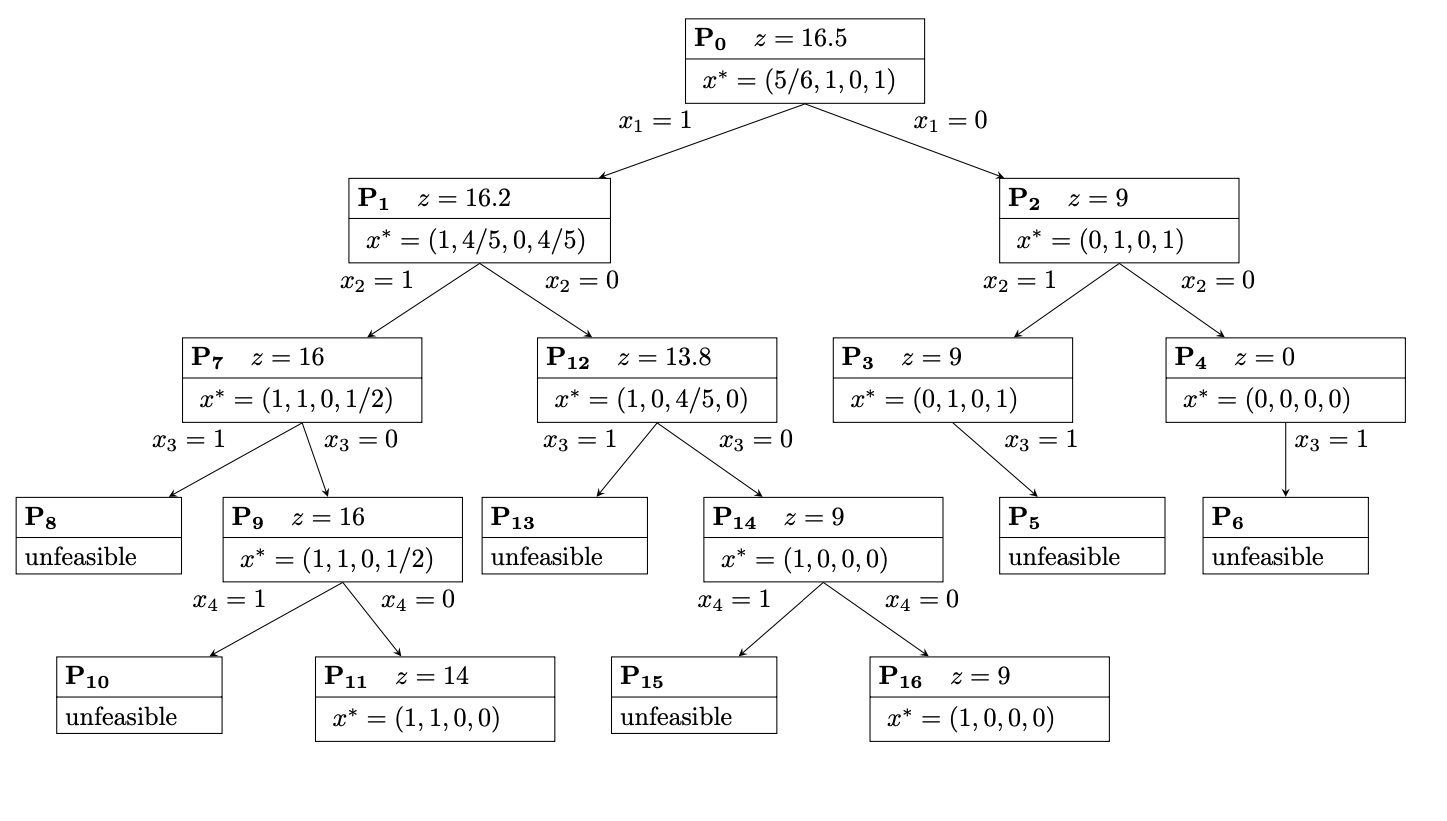
\includegraphics[width=7.29167in,height=\textheight]{tree.png}

Suppose that the Branch and Bound (BB) algorithm applies to this
problem. Also, let's suppose that the algorithm visits the sub-problems
in the following order P0 , P1 , . . . , P16. Clearly, the algorithm
does not visit all nodes.

\textbf{1) Determine the nodes that will be visited by the BB algorithm
and for each of them get the upper and lower limit deduced by the
algorithm in the execution.}

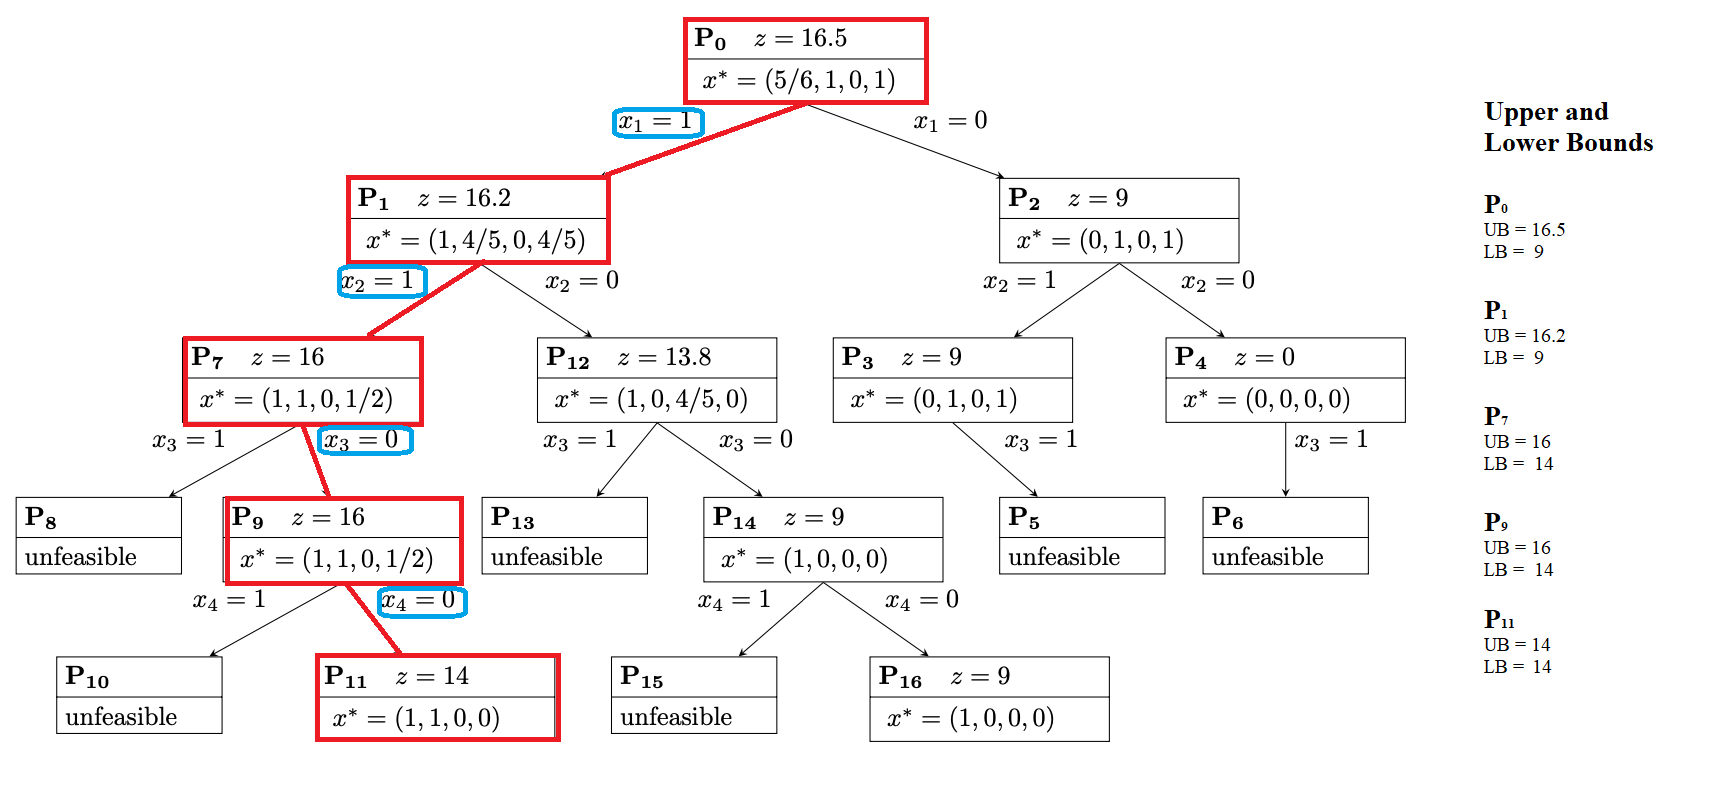
\includegraphics[width=8.33333in,height=\textheight]{BranchTree.png}

The upper bounds are obtained using relaxed solutions, and lower bounds
by rounding down the variables and subsequently calculating the value of
the objective function, as recommended on page C-5 in the
\href{http://web.tecnico.ulisboa.pt/mcasquilho/compute/_linpro/TaylorB_module_c.pdf}{following
textbook}.

\textbf{2) Solve the problem with an ILP solver and check the value of
the objective function matches the one found at point 1.}

\hypertarget{model}{%
\subsubsection{Model}\label{model}}

\begin{Shaded}
\begin{Highlighting}[]
\KeywordTok{library}\NormalTok{(lpSolveAPI)}

\NormalTok{model =}\StringTok{ }\KeywordTok{make.lp}\NormalTok{(}\DecValTok{0}\NormalTok{,}\DecValTok{4}\NormalTok{)}

\KeywordTok{name.lp}\NormalTok{(model, }\StringTok{"Problem 1"}\NormalTok{)}

\KeywordTok{lp.control}\NormalTok{(model, }\DataTypeTok{sense =} \StringTok{"max"}\NormalTok{)}

\KeywordTok{set.objfn}\NormalTok{(model, }\DataTypeTok{obj =} \KeywordTok{c}\NormalTok{(}\DecValTok{9}\NormalTok{,}\DecValTok{5}\NormalTok{,}\DecValTok{6}\NormalTok{,}\DecValTok{4}\NormalTok{))}
\end{Highlighting}
\end{Shaded}

\hypertarget{contraints}{%
\subsubsection{Contraints}\label{contraints}}

\begin{Shaded}
\begin{Highlighting}[]
\KeywordTok{add.constraint}\NormalTok{ (model,}
               \DataTypeTok{xt =} \KeywordTok{c}\NormalTok{(}\DecValTok{6}\NormalTok{,}\DecValTok{3}\NormalTok{,}\DecValTok{5}\NormalTok{,}\DecValTok{2}\NormalTok{),}
               \DataTypeTok{type =} \StringTok{"<="}\NormalTok{,}
               \DataTypeTok{rhs =} \DecValTok{10}\NormalTok{,}
               \DataTypeTok{indices =} \KeywordTok{c}\NormalTok{(}\DecValTok{1}\NormalTok{,}\DecValTok{2}\NormalTok{,}\DecValTok{3}\NormalTok{,}\DecValTok{4}\NormalTok{))}

\KeywordTok{add.constraint}\NormalTok{ (model,}
               \DataTypeTok{xt =} \KeywordTok{c}\NormalTok{(}\DecValTok{1}\NormalTok{,}\DecValTok{1}\NormalTok{),}
               \DataTypeTok{type =} \StringTok{"<="}\NormalTok{,}
               \DataTypeTok{rhs =} \DecValTok{1}\NormalTok{,}
               \DataTypeTok{indices =} \KeywordTok{c}\NormalTok{(}\DecValTok{3}\NormalTok{,}\DecValTok{4}\NormalTok{))}

\KeywordTok{add.constraint}\NormalTok{ (model,}
               \DataTypeTok{xt =} \KeywordTok{c}\NormalTok{(}\OperatorTok{-}\DecValTok{1}\NormalTok{,}\DecValTok{1}\NormalTok{),}
               \DataTypeTok{type =} \StringTok{"<="}\NormalTok{,}
               \DataTypeTok{rhs =} \DecValTok{0}\NormalTok{,}
               \DataTypeTok{indices =} \KeywordTok{c}\NormalTok{(}\DecValTok{1}\NormalTok{,}\DecValTok{3}\NormalTok{))}

\KeywordTok{add.constraint}\NormalTok{ (model,}
               \DataTypeTok{xt =} \KeywordTok{c}\NormalTok{(}\OperatorTok{-}\DecValTok{1}\NormalTok{,}\DecValTok{1}\NormalTok{),}
               \DataTypeTok{type =} \StringTok{"<="}\NormalTok{,}
               \DataTypeTok{rhs =} \DecValTok{0}\NormalTok{,}
               \DataTypeTok{indices =} \KeywordTok{c}\NormalTok{(}\DecValTok{2}\NormalTok{,}\DecValTok{4}\NormalTok{))}

\KeywordTok{set.type}\NormalTok{(model, }\KeywordTok{c}\NormalTok{(}\DecValTok{1}\OperatorTok{:}\DecValTok{4}\NormalTok{), }\StringTok{"binary"}\NormalTok{) }\CommentTok{# x1, x2, x3, x4 in \{0,1\}}
\end{Highlighting}
\end{Shaded}

\hypertarget{solution}{%
\subsubsection{Solution}\label{solution}}

\begin{Shaded}
\begin{Highlighting}[]
\KeywordTok{solve}\NormalTok{ (model)}
\end{Highlighting}
\end{Shaded}

\begin{verbatim}
## [1] 0
\end{verbatim}

\begin{Shaded}
\begin{Highlighting}[]
\KeywordTok{get.objective}\NormalTok{(model)}
\end{Highlighting}
\end{Shaded}

\begin{verbatim}
## [1] 14
\end{verbatim}

\begin{Shaded}
\begin{Highlighting}[]
\KeywordTok{get.variables}\NormalTok{(model)}
\end{Highlighting}
\end{Shaded}

\begin{verbatim}
## [1] 1 1 0 0
\end{verbatim}

The objective function, as well as the values of decision variables,
obtained by solving the model are the same as those obtained by solving
the the point one, i.e.: \[
\begin{aligned}
&Z = 14 ,
&x_{1} = 1,\:\: \: \:\: \: &x_{2} = 1,
&x_{3} = 0, \:\: \:\:\: \:
&x_{4} = 0 \\
\end{aligned}
\]

\hypertarget{problem-2}{%
\subsection{Problem 2}\label{problem-2}}

SunNet is a residential Internet Service Provider (ISP) in the central
Florida area. Presently, the company operates one centralized facility
that all of its clients call into for Internet access.

To improve service, the company is planning to open three satellite
offices in the cities of Pine Hills, Eustis, and Sanford. The company
has identified five different regions to be serviced by these three
offices. The following table summarizes the number of customers in each
region, the service capacity at each office, and the monthly average
cost per customer for providing the service to each region from each
office. Table entries of ``n.a.'' indicate infeasible region-to-service
center combinations.

SunNet would like to determine how many customers from each region to
assign to each service center to minimize the total cost.

\[
\begin{array}{lllll}
\text { Region } & \text { Pine Hills } & \text { Eustis } & \text { Sanford } & \text { Customers } \\ 
1 & \$ 6.50 & \$ 7.50 & \text { n.a. } & 30,000 \\ 
2 & \$ 7.00 & \$ 8.00 & \text { n.a. } & 40,000 \\ 
3 & \$ 8.25 & \$ 7.25 & \$ 6.75 & 25,000 \\ 
4 & \text { n.a. } & \$ 7.75 & \$ 7.00 & 35,000 \\ 
5 & \text { n.a. } & \$ 7.50 & \$ 6.75 & 33,000 \\ 
\hline
\text { Capacity } & 60,000 & 70,000 & 40,000 & 
\end{array}
\] \textbf{1) Draw a network flow model to represent this problem.}

\hypertarget{network-flow-model-graph}{%
\subsubsection{Network Flow Model
Graph}\label{network-flow-model-graph}}

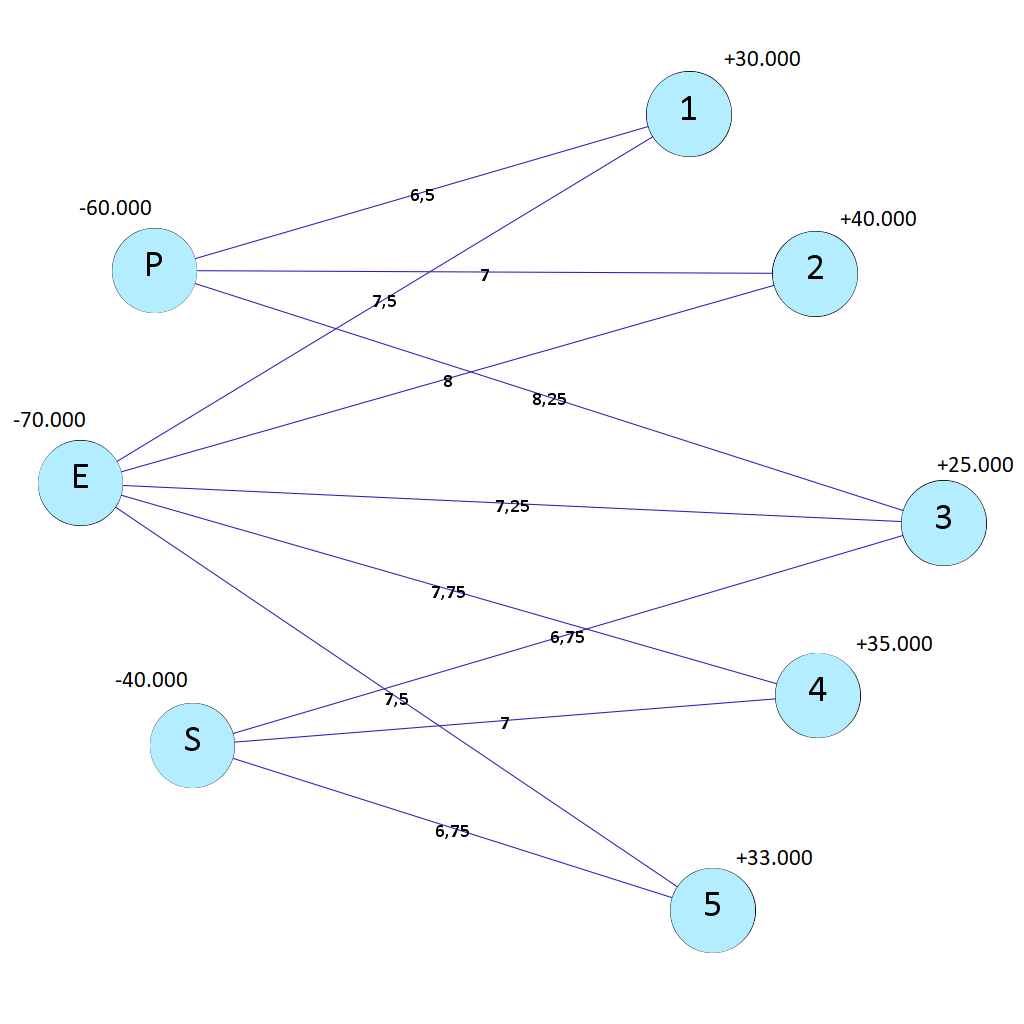
\includegraphics{graph.png}

\textbf{2) Implement your model and solve it.}

\hypertarget{model-1}{%
\subsubsection{Model:}\label{model-1}}

\hypertarget{decision-variables}{%
\paragraph{Decision Variables}\label{decision-variables}}

\(x_{i,j}\) number of clients supplied from provider i to region j.

\(i \in \{p,e,s\},\) \(j \in \{1,2,3,4,5\}\).

\hypertarget{objective-function}{%
\paragraph{Objective Function}\label{objective-function}}

\[   min: \;  6.5\,x_{p1} + 7\,x_{p2} + 8.25 \,x_{p3}\\ 
 + 7.5 \,x_{e1} + 8 \,x_{e2} + 7.25 \,x_{e3} + 7.75 \,x_{e4} + 7.5 \,x_{e5}\\
+ 6.75 \,x_{s3} + 7 \,x_{s4} + 6.75 \,x_{s5}\]

\hypertarget{constraints}{%
\paragraph{Constraints}\label{constraints}}

\textbf{Supply constraints}

\[\begin{align}
\sum_{j=1}^{3} x_{pj} \le 60000\\ 
\sum_{j=1}^{5} x_{ej} \le 70000\\
\sum_{j=3}^{5} x_{sj} \le 40000\\
\end{align}\\\]

\textbf{Demand constraints} \[\begin{align}
\sum_{i \in \{p,e\}} x_{i1} = 30000\\
\sum_{i \in \{p,e\}} x_{i2} = 40000\\
\sum_{i \in \{p,e,s\}} x_{i3} = 25000\\
\sum_{i \in \{e,s\}} x_{i4} = 35000\\
\sum_{i \in \{e,s\}} x_{i5} = 30000\\
\end{align}\\\]

In addition, the decision variables have to be integers and non
negative: \[\begin{align}
x_{ij} \in Z\\
x_{ij} \ge 0
\end{align}
\\\]

\begin{Shaded}
\begin{Highlighting}[]
\NormalTok{edges <-}\StringTok{ }\KeywordTok{data.frame}\NormalTok{(}\DataTypeTok{index_i=}  \KeywordTok{c}\NormalTok{(}\StringTok{"p"}\NormalTok{,}\StringTok{"p"}\NormalTok{,}\StringTok{"p"}\NormalTok{,  }\StringTok{"e"}\NormalTok{,}\StringTok{"e"}\NormalTok{,}\StringTok{"e"}\NormalTok{,}\StringTok{"e"}\NormalTok{,}\StringTok{"e"}\NormalTok{,  }\StringTok{"s"}\NormalTok{,}\StringTok{"s"}\NormalTok{,}\StringTok{"s"}\NormalTok{ ),}
                     \DataTypeTok{index_j =}\KeywordTok{c}\NormalTok{( }\DecValTok{1}\NormalTok{,  }\DecValTok{2}\NormalTok{,  }\DecValTok{3}\NormalTok{,    }\DecValTok{1}\NormalTok{,  }\DecValTok{2}\NormalTok{,  }\DecValTok{3}\NormalTok{,  }\DecValTok{4}\NormalTok{,  }\DecValTok{5}\NormalTok{,    }\DecValTok{3}\NormalTok{,  }\DecValTok{4}\NormalTok{,  }\DecValTok{5}\NormalTok{),}
                     \DataTypeTok{coeff =} \KeywordTok{c}\NormalTok{ (}\FloatTok{6.5}\NormalTok{,}\DecValTok{7}\NormalTok{, }\FloatTok{8.25}\NormalTok{, }\FloatTok{7.5}\NormalTok{, }\DecValTok{8}\NormalTok{, }\FloatTok{7.25}\NormalTok{,}\FloatTok{7.75}\NormalTok{,}\FloatTok{7.5}\NormalTok{, }\FloatTok{6.75}\NormalTok{,}\DecValTok{7}\NormalTok{,}\FloatTok{6.75}\NormalTok{))}

\NormalTok{edges}

\NormalTok{model <-}\StringTok{ }\KeywordTok{make.lp}\NormalTok{(}\DecValTok{0}\NormalTok{,}\DecValTok{11}\NormalTok{)}

\KeywordTok{name.lp}\NormalTok{(model, }\StringTok{"Problem 2"}\NormalTok{)}

\KeywordTok{lp.control}\NormalTok{(model, }\DataTypeTok{sense=}\StringTok{"min"}\NormalTok{)}

\KeywordTok{set.objfn}\NormalTok{(model, edges}\OperatorTok{$}\NormalTok{coeff)}

\CommentTok{# CONSTRAINTS}

\CommentTok{## SUPPLY CONSTRAINTS}

\KeywordTok{add.constraint}\NormalTok{(model,}
               \DataTypeTok{xt =} \KeywordTok{c}\NormalTok{(}\DecValTok{1}\NormalTok{,}\DecValTok{1}\NormalTok{,}\DecValTok{1}\NormalTok{),}
               \DataTypeTok{type =} \StringTok{"<="}\NormalTok{,}
               \DataTypeTok{rhs =} \DecValTok{60000}\NormalTok{,}
               \DataTypeTok{indices =} \KeywordTok{c}\NormalTok{(}\DecValTok{1}\NormalTok{,}\DecValTok{2}\NormalTok{,}\DecValTok{3}\NormalTok{)) }\CommentTok{# Supply from P}

\KeywordTok{add.constraint}\NormalTok{(model,}
               \DataTypeTok{xt =} \KeywordTok{c}\NormalTok{(}\DecValTok{1}\NormalTok{,}\DecValTok{1}\NormalTok{,}\DecValTok{1}\NormalTok{,}\DecValTok{1}\NormalTok{,}\DecValTok{1}\NormalTok{),}
               \DataTypeTok{type =} \StringTok{"<="}\NormalTok{,}
               \DataTypeTok{rhs =} \DecValTok{70000}\NormalTok{,}
               \DataTypeTok{indices =} \KeywordTok{c}\NormalTok{(}\DecValTok{4}\NormalTok{,}\DecValTok{5}\NormalTok{,}\DecValTok{6}\NormalTok{,}\DecValTok{7}\NormalTok{,}\DecValTok{8}\NormalTok{)) }\CommentTok{# Supply from E}

\KeywordTok{add.constraint}\NormalTok{(model,}
               \DataTypeTok{xt =} \KeywordTok{c}\NormalTok{(}\DecValTok{1}\NormalTok{,}\DecValTok{1}\NormalTok{,}\DecValTok{1}\NormalTok{),}
               \DataTypeTok{type =} \StringTok{"<="}\NormalTok{,}
               \DataTypeTok{rhs =} \DecValTok{40000}\NormalTok{,}
               \DataTypeTok{indices =} \KeywordTok{c}\NormalTok{(}\DecValTok{9}\NormalTok{,}\DecValTok{10}\NormalTok{,}\DecValTok{11}\NormalTok{)) }\CommentTok{# Supply from S}

\CommentTok{## DEMAND CONSTRAINTS}

\KeywordTok{add.constraint}\NormalTok{(model,}
               \DataTypeTok{xt =} \KeywordTok{c}\NormalTok{(}\DecValTok{1}\NormalTok{,}\DecValTok{1}\NormalTok{),}
               \DataTypeTok{type =} \StringTok{"="}\NormalTok{,}
               \DataTypeTok{rhs =} \DecValTok{30000}\NormalTok{,}
               \DataTypeTok{indices =} \KeywordTok{c}\NormalTok{(}\DecValTok{1}\NormalTok{,}\DecValTok{4}\NormalTok{)) }\CommentTok{# Demand region 1}

\KeywordTok{add.constraint}\NormalTok{(model,}
               \DataTypeTok{xt =} \KeywordTok{c}\NormalTok{(}\DecValTok{1}\NormalTok{,}\DecValTok{1}\NormalTok{),}
               \DataTypeTok{type =} \StringTok{"="}\NormalTok{,}
               \DataTypeTok{rhs =} \DecValTok{40000}\NormalTok{,}
               \DataTypeTok{indices =} \KeywordTok{c}\NormalTok{(}\DecValTok{2}\NormalTok{,}\DecValTok{5}\NormalTok{)) }\CommentTok{# Demand region 2}

\KeywordTok{add.constraint}\NormalTok{(model,}
               \DataTypeTok{xt =} \KeywordTok{c}\NormalTok{(}\DecValTok{1}\NormalTok{,}\DecValTok{1}\NormalTok{,}\DecValTok{1}\NormalTok{),}
               \DataTypeTok{type =} \StringTok{"="}\NormalTok{,}
               \DataTypeTok{rhs =} \DecValTok{25000}\NormalTok{,}
               \DataTypeTok{indices =} \KeywordTok{c}\NormalTok{(}\DecValTok{3}\NormalTok{,}\DecValTok{6}\NormalTok{,}\DecValTok{9}\NormalTok{)) }\CommentTok{# Demand region 3}

\KeywordTok{add.constraint}\NormalTok{(model,}
               \DataTypeTok{xt =} \KeywordTok{c}\NormalTok{(}\DecValTok{1}\NormalTok{,}\DecValTok{1}\NormalTok{),}
               \DataTypeTok{type =} \StringTok{"="}\NormalTok{,}
               \DataTypeTok{rhs =} \DecValTok{35000}\NormalTok{,}
               \DataTypeTok{indices =} \KeywordTok{c}\NormalTok{(}\DecValTok{7}\NormalTok{,}\DecValTok{10}\NormalTok{)) }\CommentTok{# Demand region 4}

\KeywordTok{add.constraint}\NormalTok{(model,}
               \DataTypeTok{xt =} \KeywordTok{c}\NormalTok{(}\DecValTok{1}\NormalTok{,}\DecValTok{1}\NormalTok{),}
               \DataTypeTok{type =} \StringTok{"="}\NormalTok{,}
               \DataTypeTok{rhs =} \DecValTok{33000}\NormalTok{,}
               \DataTypeTok{indices =} \KeywordTok{c}\NormalTok{(}\DecValTok{8}\NormalTok{,}\DecValTok{11}\NormalTok{)) }\CommentTok{# Demand region 5}


\KeywordTok{set.type}\NormalTok{ (model, }\KeywordTok{cbind}\NormalTok{(edges}\OperatorTok{$}\NormalTok{index_i,edges}\OperatorTok{$}\NormalTok{index_j), }\StringTok{"integer"}\NormalTok{)}

\KeywordTok{set.bounds}\NormalTok{(model,}\KeywordTok{c}\NormalTok{(}\KeywordTok{rep}\NormalTok{(}\DecValTok{0}\NormalTok{,}\DecValTok{11}\NormalTok{)))}

\KeywordTok{solve}\NormalTok{(model)}
\end{Highlighting}
\end{Shaded}

\textbf{3) What is the optimal solution?}

\hypertarget{optimal-solution}{%
\subsubsection{Optimal solution}\label{optimal-solution}}

The amount of the total cost for the SunNet is 1155000.

\begin{Shaded}
\begin{Highlighting}[]
\KeywordTok{get.objective}\NormalTok{(model)}
\end{Highlighting}
\end{Shaded}

\begin{verbatim}
## [1] 1155000
\end{verbatim}

The number of customers from each region assigned to each service center
in order to minimize the cost is as follows:

\begin{Shaded}
\begin{Highlighting}[]
\NormalTok{v <-}\StringTok{ }\KeywordTok{get.variables}\NormalTok{(model); v}
\end{Highlighting}
\end{Shaded}

\begin{verbatim}
##  [1] 20000 40000     0 10000     0 25000     0 28000     0 35000  5000
\end{verbatim}

\begin{Shaded}
\begin{Highlighting}[]
\NormalTok{res<-}\KeywordTok{cbind}\NormalTok{(edges, v)[}\KeywordTok{c}\NormalTok{(}\StringTok{"index_i"}\NormalTok{, }\StringTok{"index_j"}\NormalTok{, }\StringTok{"v"}\NormalTok{)]}

\NormalTok{res[res}\OperatorTok{$}\NormalTok{v }\OperatorTok{!=}\StringTok{'0'}\NormalTok{,]}
\end{Highlighting}
\end{Shaded}

\begin{verbatim}
##    index_i index_j     v
## 1        p       1 20000
## 2        p       2 40000
## 4        e       1 10000
## 6        e       3 25000
## 8        e       5 28000
## 10       s       4 35000
## 11       s       5  5000
\end{verbatim}

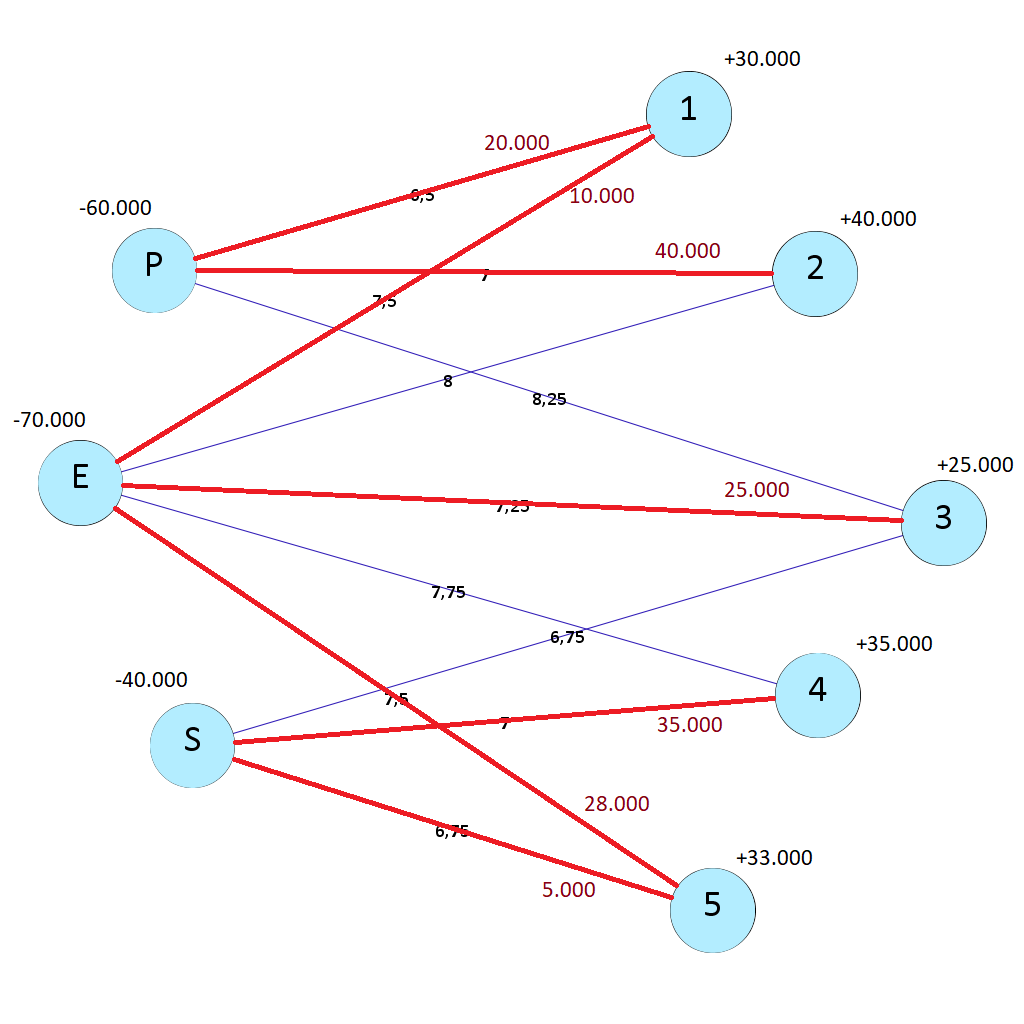
\includegraphics{graph-solved.png}

\end{document}
